\section{Results}
\label{sec:results}

\subsection{Descriptive Statistics}
\label{sec:results:desc}

Table~\ref{tab:desc_stats} summarises the BAFU~2219 annual maxima. GLOF years show a
mean \SI{70}{\percent} above non-GLOF years (\SI{29.35}{m^3\per s}
vs.\ \SI{17.28}{m^3\per s}), driven largely by the 2018 event. The relative gap is
smaller in the GRDC daily-mean series (\SI{39}{\percent}), consistent with daily
averaging dampening brief storm peaks.

\begin{table}[H]
  \centering
  \caption{Descriptive statistics of the annual maximum series (1944--2025, BAFU~2219
           extended AMS combining Monatsmaxima 1944--1973 and Tagesmaxima 1974--2025).}
  \label{tab:desc_stats}
  \begin{tabular}{lrrr}
    \toprule
    & Full series & Non-GLOF years & GLOF years (2011--2018) \\
    \midrule
    $n$                        & 82   & 74   & 8    \\
    Mean [\si{m^3\per s}]      & 18.46 & 17.28 & 29.35 \\
    Std  [\si{m^3\per s}]      &  7.51 &  5.55 & 13.45 \\
    Median [\si{m^3\per s}]    & 16.41 & 16.09 & 27.13 \\
    Min / Max [\si{m^3\per s}] & 9.89 / 56.90 & 9.89 / 34.67 & 15.55 / 56.90 \\
    \bottomrule
  \end{tabular}
\end{table}

\subsection{GLOF Contribution to Annual Maxima}
\label{sec:results:glof_contribution}

Table~\ref{tab:glof_combined} reports the annual maximum, its implied return period under
the reference GEV, and whether the $\pm 5$-day masking window captures the annual maximum
for each GLOF year, for both discharge records.

\begin{table}[H]
  \centering
  \small
  \caption{Annual maxima during the GLOF period 2011--2018 under daily maximum discharge
           (BAFU~2219) and daily mean discharge (GRDC). The implied return period $\hat{T}$
           is computed under the respective pre-GLOF reference GEV (1944--2010 for both
           datasets). ``GLOF = max?'' indicates whether the $\pm 5$-day masking window
           contains the annual maximum.}
  \label{tab:glof_combined}
  \begin{tabular}{ccrrcrrcc}
    \toprule
    & & \multicolumn{3}{c}{Daily max.\ (BAFU 2219)} & \multicolumn{3}{c}{Daily mean (GRDC)} \\
    \cmidrule(lr){3-5}\cmidrule(lr){6-8}
    Year & GLOF date & $Q_\text{ann}$ & $\hat{T}$ & GLOF & $Q_\text{ann}$ & $\hat{T}$ & GLOF \\
         &           & [\si{m^3\per s}] & [yr] & =max? & [\si{m^3\per s}] & [yr] & =max? \\
    \midrule
    2011 & 27 Jul & 27.09 &   17.0 & No  & 15.08 &  17.4 & No  \\
    2012 & 16 Jul & 19.12 &    3.8 & Yes & 14.56 &  13.6 & Yes \\
    2013 &  2 Aug & 20.59 &    5.0 & Yes & 14.99 &  16.6 & Yes \\
    2014 &  7 Aug & 40.48 &  126.7 & No  & 21.09 & 220.0 & Yes \\
    2015 &  1 Aug & 15.55 &    1.9 & No  & 10.11 &   1.6 & Yes \\
    2016 & 28 Aug & 27.16 &   17.2 & Yes & 13.97 &  10.2 & No  \\
    2017 & 19 Jul & 27.95 &   19.7 & No  & 13.94 &  10.0 & Yes \\
    2018 & 27 Jul & 56.90 &  788.8 & Yes & 19.24 & 107.1 & Yes \\
    \midrule
    \multicolumn{2}{c}{GLOF = ann.\ max (of 8 GLOF yrs)} & \multicolumn{3}{c}{4 / 8} & \multicolumn{3}{c}{6 / 8} \\
    \bottomrule
  \end{tabular}
\end{table}

Under daily maxima, the GLOF produced the annual maximum in 4 of 8 years (2012, 2013,
2016, 2018); in the remaining four, storm floods dominated, including a
$\hat{T} \approx 127$-year event in 2014. Under daily means, GLOFs dominated in 6 of 8
years, because their sustained outflows elevate the 24-hour average above brief
convective peaks.

\subsection{GEV Parameter Estimates}
\label{sec:results:gev}

Table~\ref{tab:gev_params} shows the MLE parameter estimates. Including GLOF years shifts
$\hat{\xi}$ toward a heavier Fréchet tail in both datasets; masking restores it close to
the reference value ($\Delta\hat{\xi} = +0.091$ for BAFU~2219; $+0.069$ for GRDC). The
AIC is substantially lower for the masked than the full-series fit.

\begin{table}[H]
  \centering
  \caption{GEV MLE parameter estimates and AIC for both discharge datasets.}
  \label{tab:gev_params}
  \begin{tabular}{llrrrrl}
    \toprule
    Dataset & Series & $n$ & $\hat{\mu}$ & $\hat{\sigma}$ & $\hat{\xi}$ & AIC \\
    \midrule
    \multicolumn{7}{l}{\textit{BAFU 2219 — daily maximum [\si{m^3\per s}]}} \\[2pt]
     & Full 1944--2025        & 82 & 14.94 & 3.95 & 0.251 & 513.66 \\
     & GLOF-masked 1944--2025 & 82 & 14.76 & 3.67 & 0.203 & 497.56 \\
     & Reference 1944--2010   & 67 & 14.52 & 3.55 & 0.160 & 399.73 \\
    \midrule
    \multicolumn{7}{l}{\textit{GRDC — daily mean [\si{m^3\per s}]}} \\[2pt]
     & Full 1944--2020        & 77 & 10.211 & 1.711 & 0.170 & 346.93 \\
     & GLOF-masked 1944--2020 & 77 & 10.133 & 1.580 & 0.093 & 328.16 \\
     & Reference 1944--2010   & 67 & 10.038 & 1.542 & 0.101 & 283.54 \\
    \bottomrule
  \end{tabular}
\end{table}

\subsection{Design Quantiles}
\label{sec:results:quantiles}

Design quantiles are compared in Tables~\ref{tab:quantiles_bafu}
and~\ref{tab:quantiles_grdc}. The GLOF-inclusive 100-year quantile exceeds the masked
estimate by \SI{15.0}{\percent} for BAFU~2219 and \SI{16.1}{\percent} for GRDC, growing
to 18--20\,\% at 200 years. Masked and reference fits are closely aligned in both
datasets.

\begin{table}[H]
  \centering
  \caption{GEV design quantiles [\si{m^3\per s}] for selected return periods --- BAFU~2219
           extended AMS (1944--2025), with 95\,\% delta-method confidence intervals.}
  \label{tab:quantiles_bafu}
  \begin{tabular}{lrrrrrrr}
    \toprule
    $T$ [yr] & 2 & 5 & 10 & 20 & 50 & 100 & 200 \\
    \midrule
    Full 1944--2025      & 16.47 & 22.12 & 26.81 & 32.38 & 41.08 & 48.99 & 58.68 \\
    GLOF-masked          & 16.17 & 21.19 & 25.18 & 29.75 & 36.61 & 42.61 & 49.71 \\
    Reference 1944--2010 & 15.87 & 20.53 & 24.09 & 28.04 & 33.77 & 38.61 & 44.17 \\
    \bottomrule
  \end{tabular}
\end{table}

\begin{table}[H]
  \centering
  \caption{GEV design quantiles [\si{m^3\per s}] for selected return periods --- GRDC
           daily mean discharge.}
  \label{tab:quantiles_grdc}
  \begin{tabular}{lrrrrrrr}
    \toprule
    $T$ [yr] & 2 & 5 & 10 & 20 & 50 & 100 & 200 \\
    \midrule
    Full 1944--2020      & 10.86 & 13.13 & 14.90 & 16.82 & 19.68 & 22.14 & 24.90 \\
    GLOF-masked          & 10.72 & 12.68 & 14.09 & 15.54 & 17.57 & 19.21 & 20.95 \\
    Reference 1944--2010 & 10.61 & 12.54 & 13.93 & 15.38 & 17.41 & 19.07 & 20.83 \\
    \bottomrule
  \end{tabular}
\end{table}

\begin{figure}[H]
  \centering
  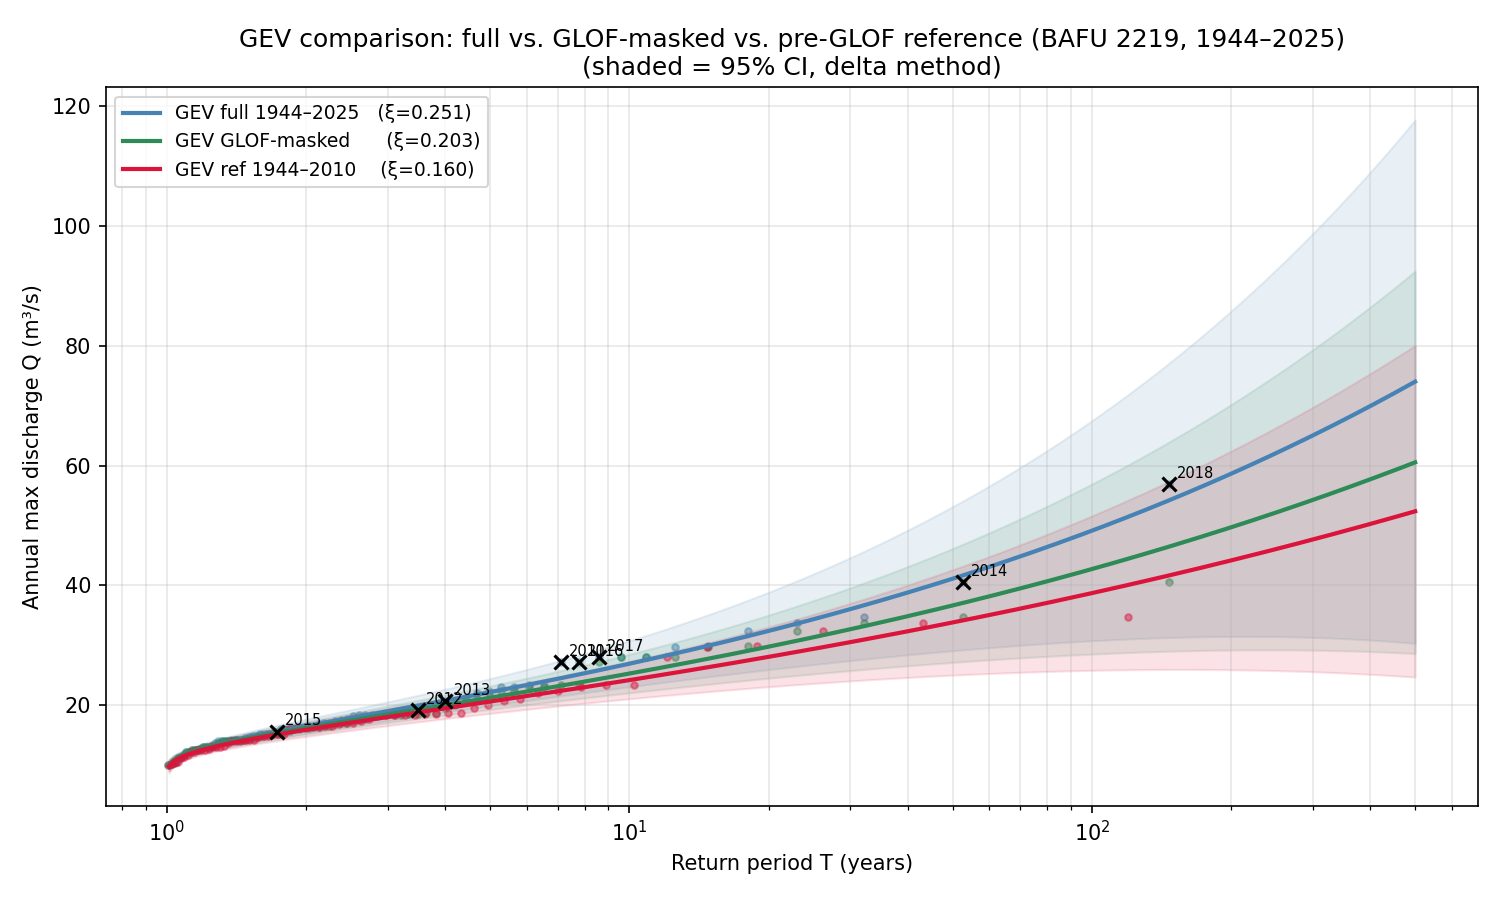
\includegraphics[width=\linewidth]{../figures_2219/02_gev/02_gev_three_curves.png}
  \caption{Return period plot for BAFU~2219 extended AMS (1944--2025): full (blue),
           GLOF-masked (green), and reference (red) GEV fits with 95\,\% delta-method
           confidence bands. Black crosses mark GLOF-year annual maxima at their empirical
           return period under the full-series fit. The 2018 event at
           $\hat{T} \approx 789$\,yr dominates the upper tail.}
  \label{fig:gev_three}
\end{figure}

\subsection{Homogeneity Tests}
\label{sec:results:tests}

\subsubsection{KS Test}

Table~\ref{tab:ks} reports the KS statistics ($n = 8$, $C_{0.05} = 0.455$). Group~A
(GLOF-inclusive) rejects $H_0$ in both datasets (BAFU~2219: $D_n = 0.610$, $p = 0.002$;
GRDC: $D_n = 0.776$, $p < 0.001$). Group~B (GLOF-masked) fails to reject in both
($D_n < 0.37$, $p > 0.19$).

\begin{table}[H]
  \centering
  \caption{KS test results: 2011--2018 peaks vs.\ pre-GLOF reference GEV (1944--2010)
           for both discharge datasets ($n = 8$; $C_{0.05} = 0.455$).}
  \label{tab:ks}
  \begin{tabular}{llcccl}
    \toprule
    Dataset & Group & $D_n$ & $C_{0.05}$ & $p$-value & Decision \\
    \midrule
    \multirow{2}{*}{BAFU 2219 (daily max.)}
      & A: GLOF-inclusive & 0.610 & 0.455 & 0.002    & Reject $H_0$ at 5\% \\
      & B: GLOF-masked    & 0.360 & 0.455 & 0.195    & Fail to reject \\
    \midrule
    \multirow{2}{*}{GRDC (daily mean)}
      & A: GLOF-inclusive & 0.776 & 0.455 & $<$0.001 & Reject $H_0$ at 5\% \\
      & B: GLOF-masked    & 0.318 & 0.455 & 0.321    & Fail to reject \\
    \bottomrule
  \end{tabular}
\end{table}

\subsubsection{Rank-Sum Test}

Table~\ref{tab:ranksum} shows the Rank-Sum results. Comparison~5a rejects $H_0$ in both
datasets. Comparison~5b fails to reject, confirming masking restores homogeneity.
Comparison~5c (pre-GLOF reference vs.\ masked GLOF-era peaks) also fails to reject
(BAFU~2219: $p = 0.172$; GRDC: $p = 0.233$).

\begin{table}[H]
  \centering
  \caption{Rank-Sum test results (two-sided, $\alpha = 0.05$) for both discharge
           datasets. Comparison~5c tests whether the masked GLOF-era peaks are consistent
           with the pre-GLOF reference.}
  \label{tab:ranksum}
  \begin{tabular}{lllccl}
    \toprule
    Dataset & & Comparison & $W$ & $p$-value & Decision \\
    \midrule
    \multirow{3}{*}{BAFU 2219}
      & 5a & GLOF-year full vs.\ non-GLOF years       & 499.0 & 0.002 & Reject $H_0$ \\
      & 5b & GLOF-year masked vs.\ non-GLOF years     & 382.0 & 0.182 & Fail to reject \\
      & 5c & Pre-GLOF ref vs.\ masked GLOF era               & 188.0 & 0.172 & Fail to reject \\
    \midrule
    \multirow{3}{*}{GRDC}
      & 5a & GLOF-year full vs.\ non-GLOF years             & 486.0 & 0.001 & Reject $H_0$ \\
      & 5b & GLOF-year masked vs.\ non-GLOF years           & 349.0 & 0.226 & Fail to reject \\
      & 5c & Pre-GLOF ref vs.\ masked GLOF era              & 198.0 & 0.233 & Fail to reject \\
    \bottomrule
  \end{tabular}
\end{table}

\begin{figure}[H]
  \centering
  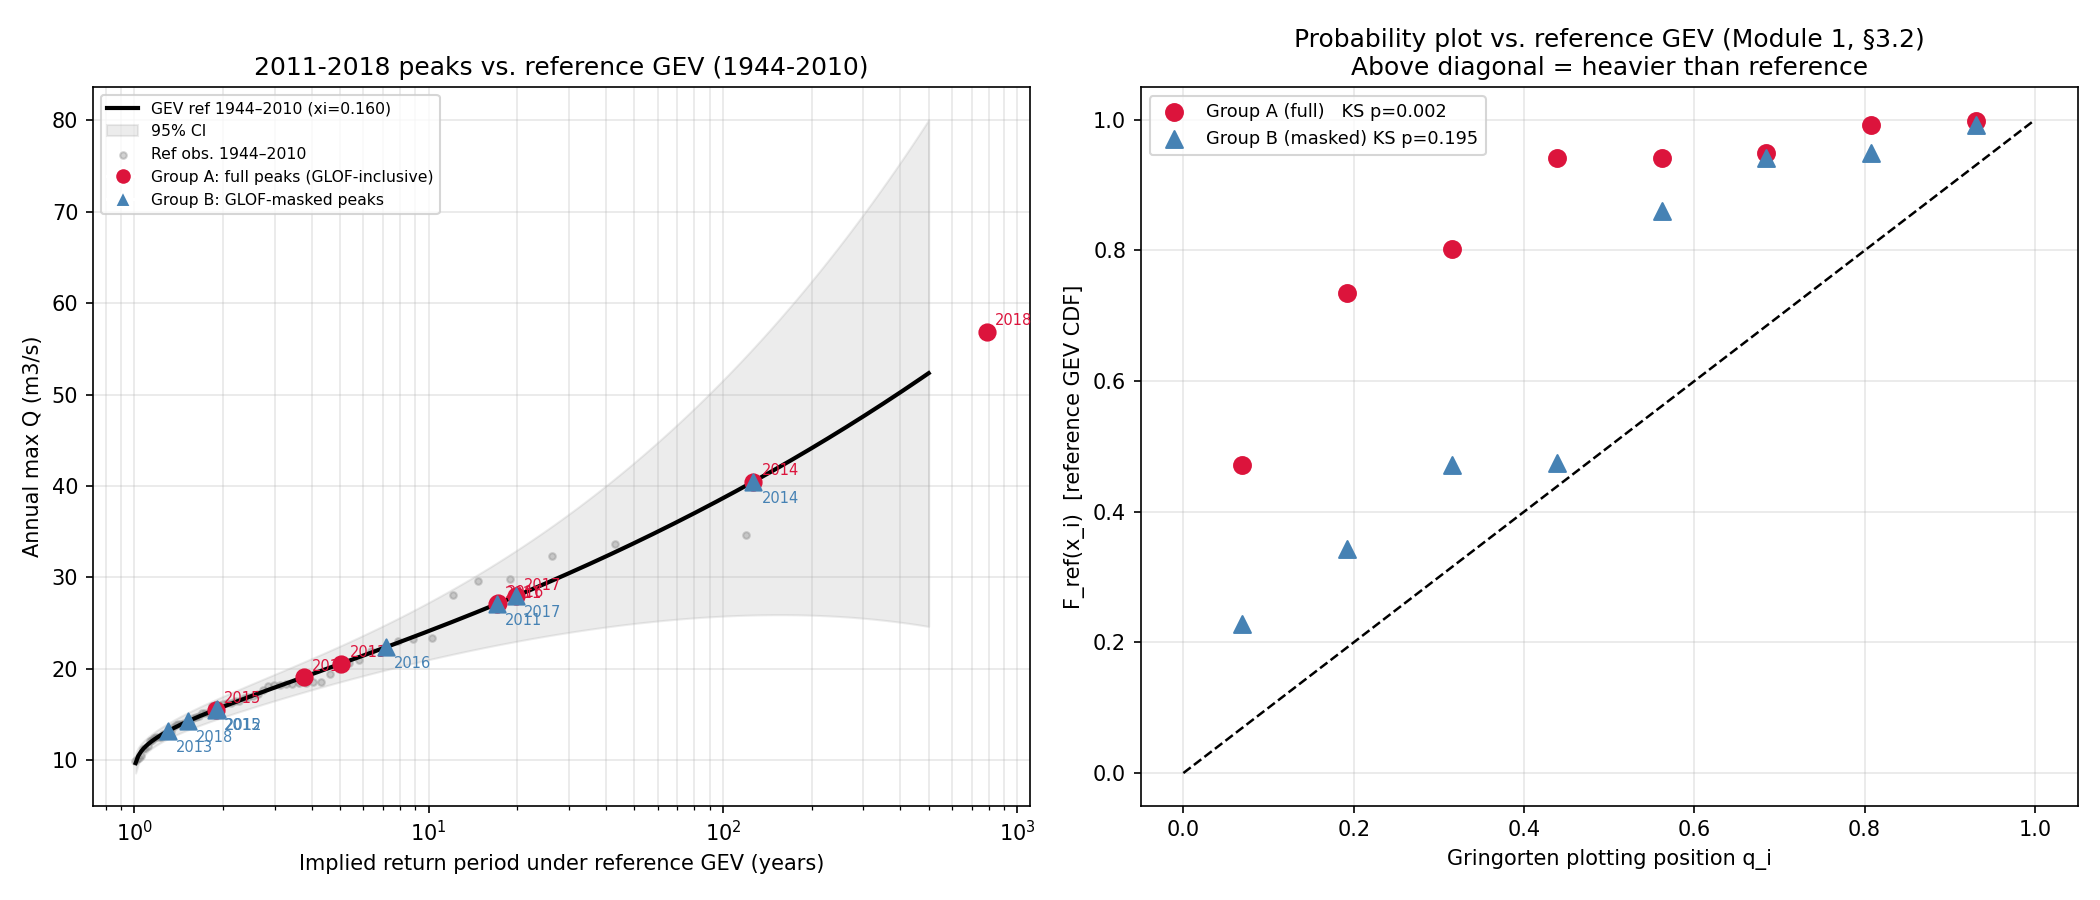
\includegraphics[width=\linewidth]{../figures_2219/03_tests/03_reference_gev_test.png}
  \caption{Left: 2011--2018 BAFU~2219 daily-maximum peaks on the reference GEV
           return-period curve (1944--2010). The 2018 GLOF-inclusive peak (crimson,
           $\hat{T} \approx 789$\,yr) dominates; after masking it drops to
           $\hat{T} \approx 1.5$\,yr (blue triangle). Right: probability plot
           (Module~1, \S3.2). Group~A lies above the diagonal almost entirely
           owing to 2018; Group~B is broadly consistent with the 1:1 line.}
  \label{fig:pp}
\end{figure}
